%!TEX root = main.tex

\subsection{Named entities extraction}

\textbf{Named entities} are proper names, quantity phrases, events, \dots There is two common difficulties when extracting NE: \textbf{variants} (USA = United States of America) and \textbf{ambiguities} (Washington).\\ To build a name tagger, there is two approches: \textbf{Hand-written} (internal evidence and external evidence) and \textbf{Automated training} (relies on tagged corpora).

Here is how automated training works:
\begin{itemize}
	\item We encode data IOB style (B: word starting entity, I: others words of entity, O: dont belong to entity);
	\item Select features from those inputs (shape features and predicitve words);
	\item Encode training set with features;
	\item Train classifier before labelling new data.
\end{itemize}

\begin{figure}[htp]
	\centering
	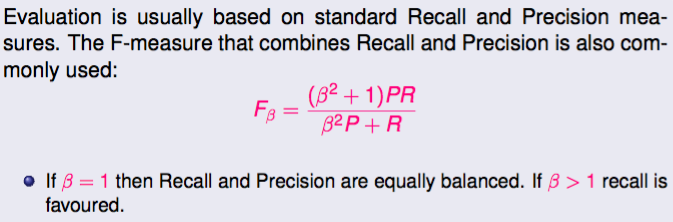
\includegraphics[scale=0.5]{images/69_eval.png}
 	\caption{Evaluation of NER system. $R = \frac{TP}{TP + FN}$ and $P = \frac{TP}{TP + FP}$.}
\end{figure}

\subsection{Relation detection}

Different kinds of relation.

\subsubsection{Hand-written extraction}

We can use regular expressions, extraction  graphs and language resources.

\subsubsection{Statistical approach}

\paragraph{Supervised}

Using hand annoted data. First step is to train a classifier that say if two NE are in relation or not. The second step is to train a classifier that label the relation based on features from the NE, words in the context and syntactic structure.

\paragraph{Semi-supervised}

Induce new patterns by bootstrapping from the initial search results from a small set of seed patterns.

\begin{figure}[htp]
	\centering
	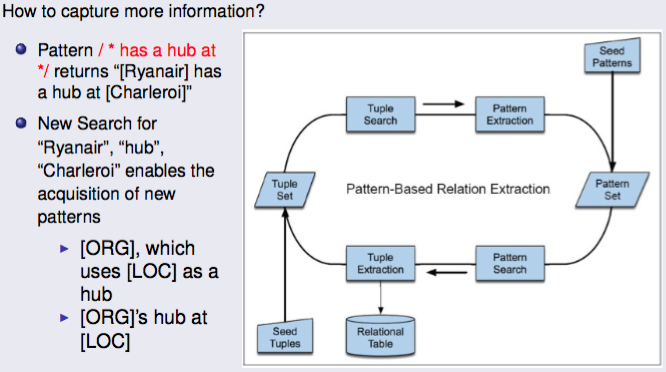
\includegraphics[scale=0.5]{images/70_example.png}
 	\caption{More information with semi-supervised learning.}
\end{figure}

\subsection{Event extraction}

Use stereotypical situation in the world. These situations can be characterized as scripts and scripts can be represented as template. The task is to fill the template.

There is somes steps: Named entities, phrase extraction, anaphora resolution (grouping same NE), pattern extraction.